\subsubsection{Design-Based Research}

Design-based research (DBR) is a research methodology aimed at improving educational practices through systematic, flexible, and iterative processes of analysis, design, development, implementation, and evaluation. It is grounded in collaboration between researchers and practitioners in real-world settings, ultimately producing design principles or theoretical contributions \parencite{wang_influence_2026}.

DBR is primarily conducted in authentic educational environments to bridge the gap between theoretical research and practical application \parencite{jong_design-based_2017}. Unlike traditional laboratory-based approaches, DBR is situated in naturalistic contexts where social interactions and environmental complexity are preserved and considered as integral parts of the research process \parencite{wang_influence_2026}.

A central feature of DBR is its iterative cycle, which consists of design, enactment, analysis, and redesign illustrated in \cref{fig:dbr_cycle}. The outputs of each cycle inform and guide subsequent cycles, enabling continuous refinement of both the intervention and the underlying theory \parencite{jong_design-based_2017}.


\begin{figure}[H]
\caption{Iterative cycle of Design-Based Research}\label{fig:dbr_cycle}
\centering
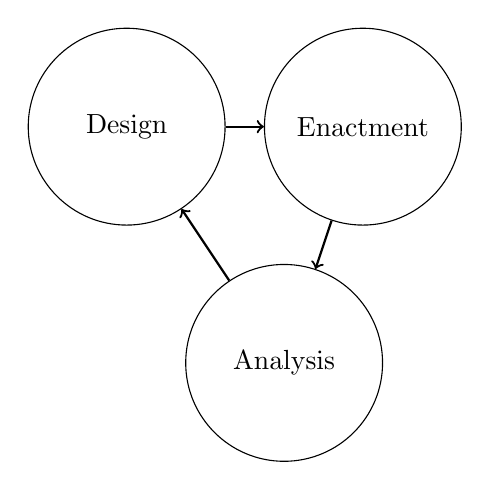
\begin{tikzpicture}[
    every node/.style={draw, circle, minimum size=2.5cm, align=center},
    arrow/.style={->, thick}
]

\node (design) at (0,0) {Design};
\node (enact) at (3,0) {Enactment};
\node (analysis) at (2,-3) {Analysis};

\draw[arrow] (design) -- (enact);
\draw[arrow] (enact) -- (analysis);
\draw[arrow] (analysis) -- (design);

\end{tikzpicture}
\end{figure}